% Appendix to the UFO camera user manual
%

\begin{appendix}

\chapter{Camera characterization}
\label{camera_char}

Camera characterization is done in IEKP using tungsten X-ray tube, and ANKA detector lab, using visible light.
Estimation of dark noise is given in \figurename~\ref{darknoise}. Camera setting for long integration time is setting the PGA value (analog gain) on address 102 to 0, which is a default value. For short integration time, PGA value is 3, which is a maximum one. Other sensor register values, unless otherwise stated, are recommended values.

\begin{figure}[ht]
\centering
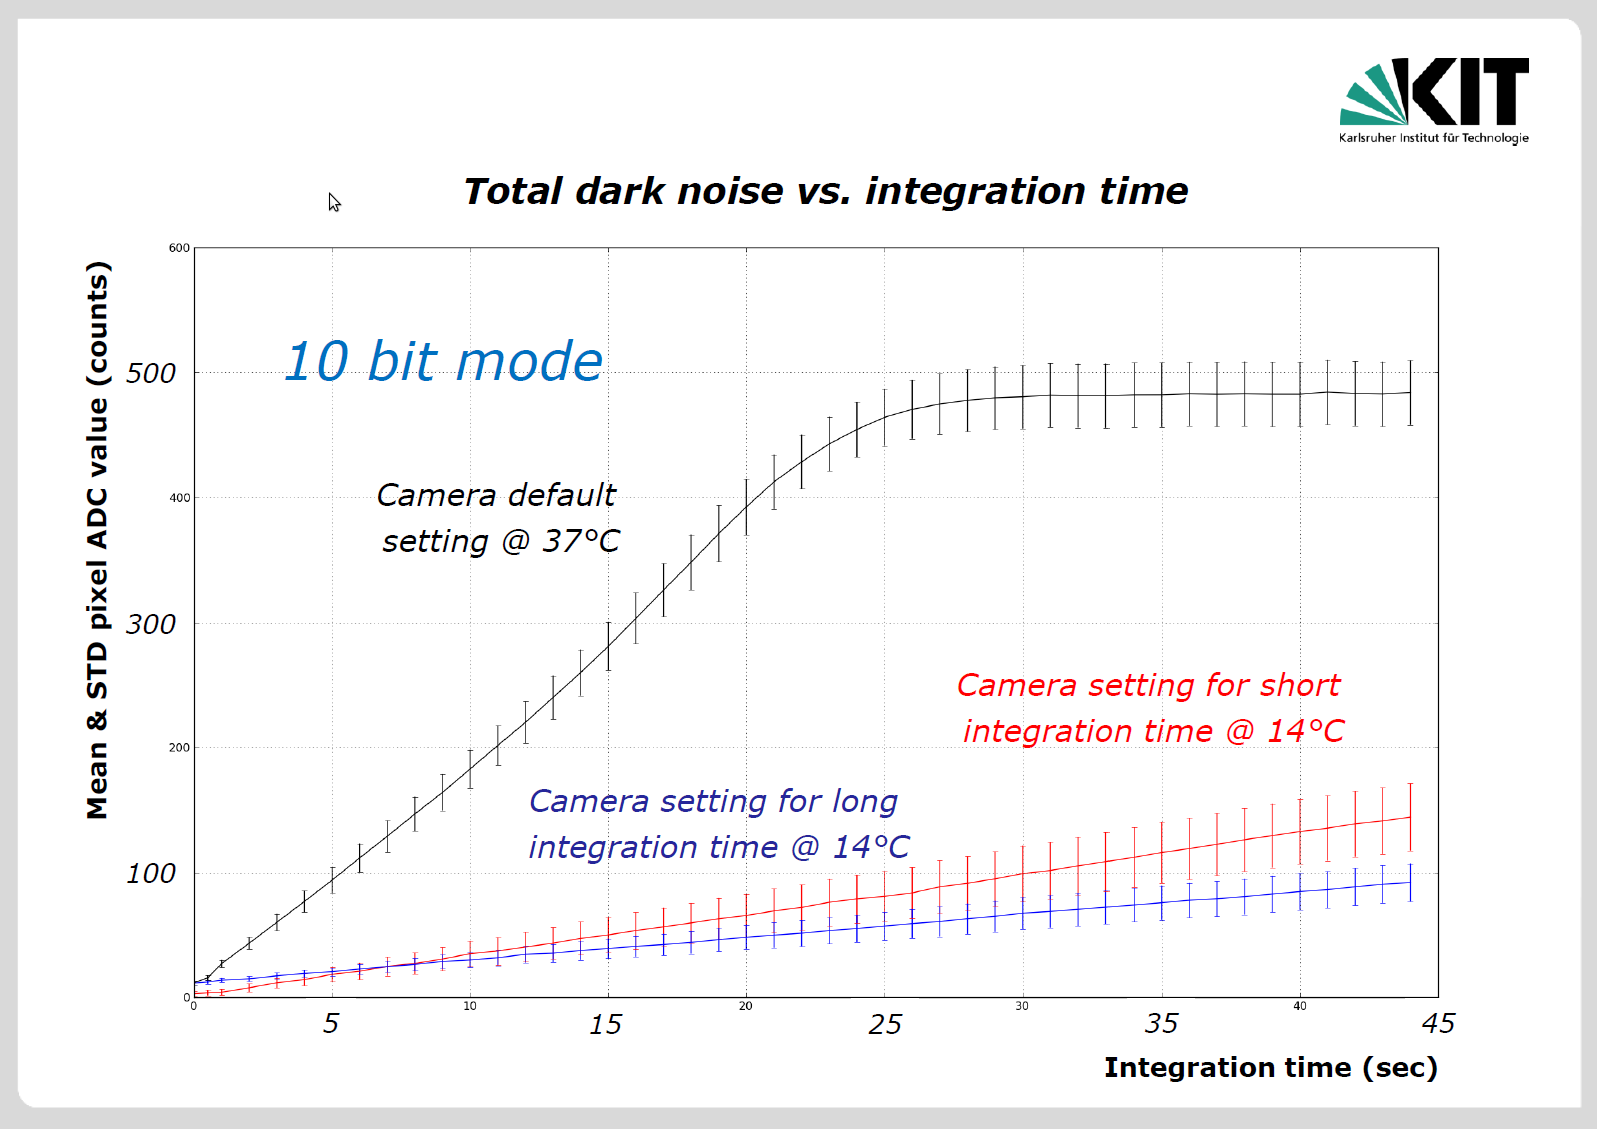
\includegraphics[width=0.70\textwidth]{images/camera_char1.png}
\caption{\label{darknoise}The total dark noise vs. integration time at different camera settings}
\end{figure}
\begin{table}[h]
\begin{center}
{\begin{tabular}{|c|c|}
\hline
Parameters & Values \\ 
\hline
Quantum efficiency &  57.41 \% \\
\hline
Dark noise  $\sigma_{d}$ &  10 $e^{-}$\\
\hline
Dynamic range & 57.22 dB \\
\hline
Conversion factor	& 7.82 $e^{-}/{DN}$ \\
\hline
\end{tabular}}
\caption{10 bit characterization of UFO camera}
\label{char_10b}
\end{center}
\end{table}



\end{appendix}

